\documentclass[tikz, border=5pt, 12pt]{standalone}
\usetikzlibrary{positioning}

% To create the figures (must have pdf2svg):
% > for i in {1..4}; do pdf2svg schematics.pdf schematics$i.svg $i; done

\begin{document}

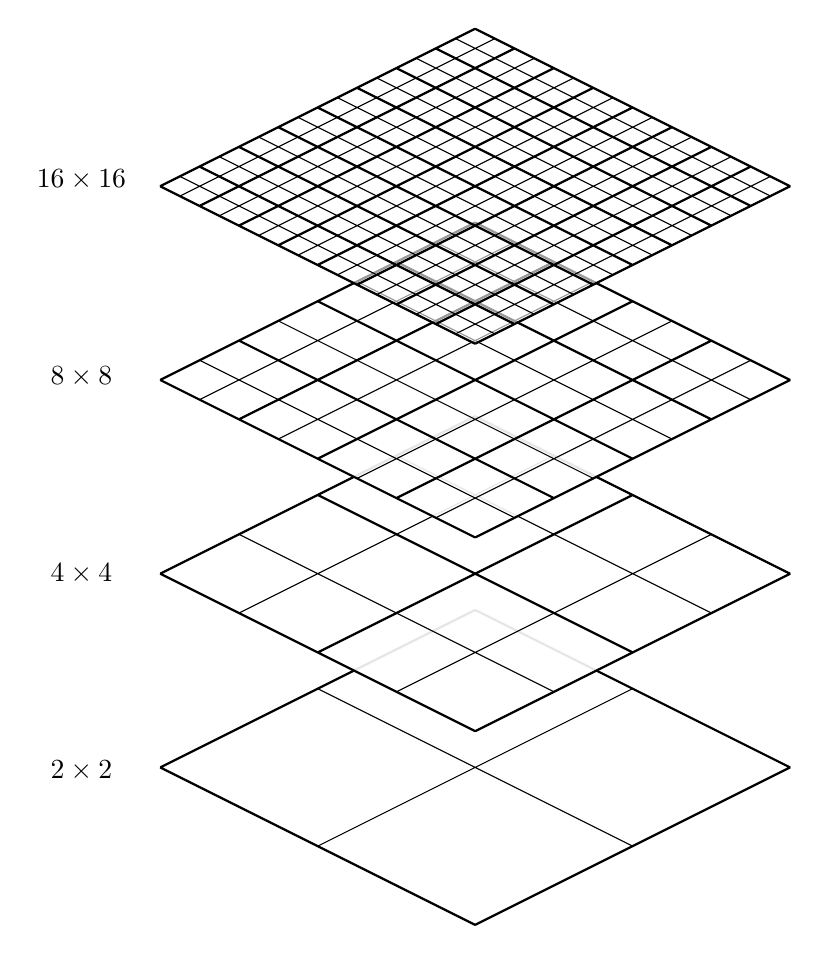
\begin{tikzpicture}
    % 2x2 Coarsest grid
    \node at (-5, -0.5) {$2\times2$};
    \begin{scope}[
            yshift=-70,every node/.append style={
            yslant=0.5,xslant=-1},yslant=0.5,xslant=-1
            ]
        \fill[white,fill opacity=0.9] (0,0) rectangle (4,4);
        \draw[step=40mm, thick] (0,0) grid (4,4);
        \draw[step=20mm] (0,0) grid (4,4);
    \end{scope}

    % 4x4
    \node at (-5, 2) {$4\times4$};
    \begin{scope}[
        yshift=0,every node/.append style={
            yslant=0.5,xslant=-1},yslant=0.5,xslant=-1
                     ]
        \fill[white,fill opacity=.9] (0,0) rectangle (4,4);
        \draw[step=20mm, thick] (0,0) grid (4,4);
        \draw[step=10mm] (0,0) grid (4,4);
    \end{scope}

    % 8x8
    \node at (-5, 4.5) {$8\times8$};
    \begin{scope}[
        yshift=70,every node/.append style={
        yslant=0.5,xslant=-1},yslant=0.5,xslant=-1
                     ]
        \fill[white,fill opacity=.9] (0,0) rectangle (4,4);
        \draw[step=10mm, thick] (0,0) grid (4,4);
        \draw[step=5mm] (0,0) grid (4,4);
    \end{scope}

    % 16x16 Finest grid
    \node at (-5, 7) {$16\times16$};
    \begin{scope}[
        yshift=140,every node/.append style={
            yslant=0.5,xslant=-1},yslant=0.5,xslant=-1
          ]
        \fill[white,fill opacity=0.6] (0,0) rectangle (4,4);
        \draw[step=5mm, thick] (0,0) grid (4,4);
        \draw[step=2.5mm] (0,0) grid (4,4);

    \end{scope}

\end{tikzpicture}

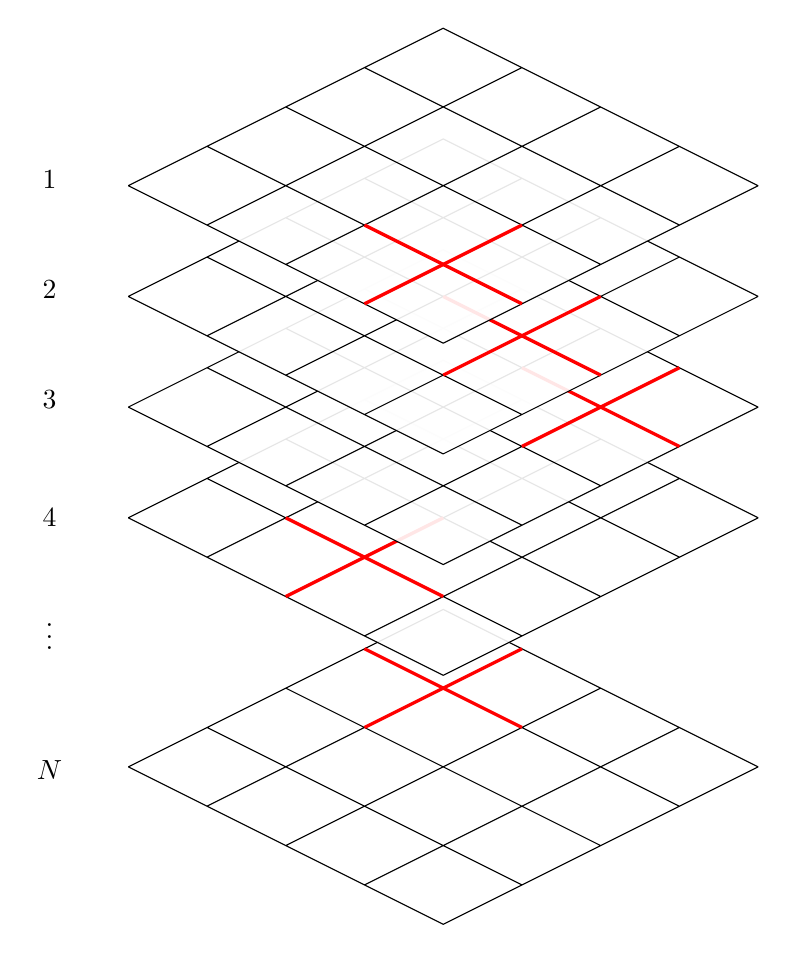
\begin{tikzpicture}

    % Nth smoothing step
    \node at (-5, -0.5) {$N$};
    \begin{scope}[
            yshift=-70,every node/.append style={
            yslant=0.5,xslant=-1},yslant=0.5,xslant=-1
            ]
        \fill[white,fill opacity=0.9] (0,0) rectangle (4,4);
        \draw[step=10mm] (0,0) grid (4,4);
        \draw[red, very thick] (3,3) -- (2,3);
        \draw[red, very thick] (3,3) -- (3,2);
        \draw[red, very thick] (3,3) -- (4,3);
        \draw[red, very thick] (3,3) -- (3,4);
    \end{scope}

    % \ldots
    \node at (-5, 1.3) {\vdots};
    \begin{scope}[
        yshift=0,every node/.append style={
            yslant=0.5,xslant=-1},yslant=0.5,xslant=-1
                     ]
    \end{scope}

    % 4nd smoothing step
    \node at (-5, 2.7) {$4$};
    \begin{scope}[
        yshift=20,every node/.append style={
        yslant=0.5,xslant=-1},yslant=0.5,xslant=-1
                     ]
        \fill[white,fill opacity=0.9] (0,0) rectangle (4,4);
        \draw[step=10mm] (0,0) grid (4,4);
        \draw[red, very thick] (1,2) -- (0,2);
        \draw[red, very thick] (1,2) -- (1,1);
        \draw[red, very thick] (1,2) -- (2,2);
        \draw[red, very thick] (1,2) -- (1,3);
    \end{scope}

    % 3nd smoothing step
    \node at (-5, 4.2) {$3$};
    \begin{scope}[
        yshift=60,every node/.append style={
        yslant=0.5,xslant=-1},yslant=0.5,xslant=-1
                     ]
        \fill[white,fill opacity=0.9] (0,0) rectangle (4,4);
        \draw[step=10mm] (0,0) grid (4,4);
        \draw[red, very thick] (3,1) -- (2,1);
        \draw[red, very thick] (3,1) -- (3,0);
        \draw[red, very thick] (3,1) -- (4,1);
        \draw[red, very thick] (3,1) -- (3,2);
    \end{scope}

    % 2nd smoothing step
    \node at (-5, 5.6) {$2$};
    \begin{scope}[
        yshift=100,every node/.append style={
        yslant=0.5,xslant=-1},yslant=0.5,xslant=-1
                     ]
        \fill[white,fill opacity=0.9] (0,0) rectangle (4,4);
        \draw[step=10mm] (0,0) grid (4,4);
        \draw[red, very thick] (2,1) -- (1,1);
        \draw[red, very thick] (2,1) -- (2,0);
        \draw[red, very thick] (2,1) -- (3,1);
        \draw[red, very thick] (2,1) -- (2,2);
    \end{scope}

    % 1st smoothing step
    \node at (-5, 7) {$1$};
    \begin{scope}[
        yshift=140,every node/.append style={
            yslant=0.5,xslant=-1},yslant=0.5,xslant=-1
          ]
        \fill[white,fill opacity=0.9] (0,0) rectangle (4,4);
        \draw[step=10mm] (0,0) grid (4,4);
        \draw[red, very thick] (1,1) -- (0,1);
        \draw[red, very thick] (1,1) -- (1,0);
        \draw[red, very thick] (1,1) -- (2,1);
        \draw[red, very thick] (1,1) -- (1,2);

    \end{scope}

\end{tikzpicture}

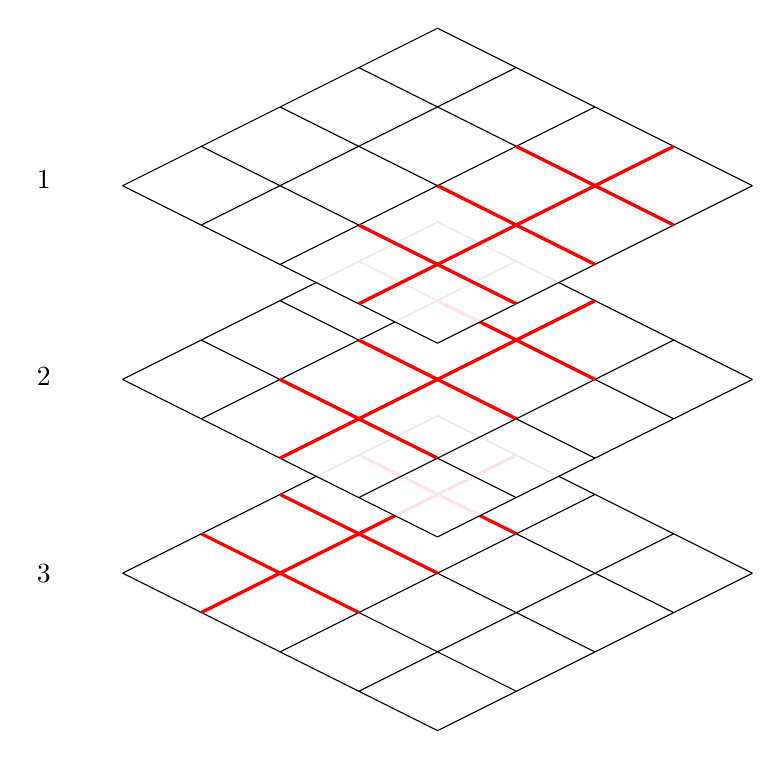
\begin{tikzpicture}

    % Nth smoothing step
    \node at (-5, 2) {$3$};
    \begin{scope}[
            yshift=0,every node/.append style={
            yslant=0.5,xslant=-1},yslant=0.5,xslant=-1
            ]
        \fill[white,fill opacity=0.9] (0,0) rectangle (4,4);
        \draw[step=10mm] (0,0) grid (4,4);
        \draw[red, very thick] (1,3) -- (0,3);
        \draw[red, very thick] (1,3) -- (1,2);
        \draw[red, very thick] (1,3) -- (2,3);
        \draw[red, very thick] (1,3) -- (1,4);
        \draw[red, very thick] (2,3) -- (2,2);
        \draw[red, very thick] (2,3) -- (3,3);
        \draw[red, very thick] (2,3) -- (2,4);
        \draw[red, very thick] (3,3) -- (3,2);
        \draw[red, very thick] (3,3) -- (4,3);
        \draw[red, very thick] (3,3) -- (3,4);
    \end{scope}

    % 2nd smoothing step
    \node at (-5, 4.5) {$2$};
    \begin{scope}[
        yshift=70,every node/.append style={
        yslant=0.5,xslant=-1},yslant=0.5,xslant=-1
                     ]
        \fill[white,fill opacity=0.9] (0,0) rectangle (4,4);
        \draw[step=10mm] (0,0) grid (4,4);
        \draw[red, very thick] (1,2) -- (0,2);
        \draw[red, very thick] (1,2) -- (1,1);
        \draw[red, very thick] (1,2) -- (2,2);
        \draw[red, very thick] (1,2) -- (1,3);
        \draw[red, very thick] (2,2) -- (2,1);
        \draw[red, very thick] (2,2) -- (3,2);
        \draw[red, very thick] (2,2) -- (2,3);
        \draw[red, very thick] (3,2) -- (3,1);
        \draw[red, very thick] (3,2) -- (4,2);
        \draw[red, very thick] (3,2) -- (3,3);
    \end{scope}

    % 1st smoothing step
    \node at (-5, 7) {$1$};
    \begin{scope}[
        yshift=140,every node/.append style={
            yslant=0.5,xslant=-1},yslant=0.5,xslant=-1
          ]
        \fill[white,fill opacity=0.9] (0,0) rectangle (4,4);
        \draw[step=10mm] (0,0) grid (4,4);
        \draw[red, very thick] (1,1) -- (0,1);
        \draw[red, very thick] (1,1) -- (1,0);
        \draw[red, very thick] (1,1) -- (2,1);
        \draw[red, very thick] (1,1) -- (1,2);
        \draw[red, very thick] (2,1) -- (2,0);
        \draw[red, very thick] (2,1) -- (3,1);
        \draw[red, very thick] (2,1) -- (2,2);
        \draw[red, very thick] (3,1) -- (3,0);
        \draw[red, very thick] (3,1) -- (4,1);
        \draw[red, very thick] (3,1) -- (3,2);

    \end{scope}

\end{tikzpicture}

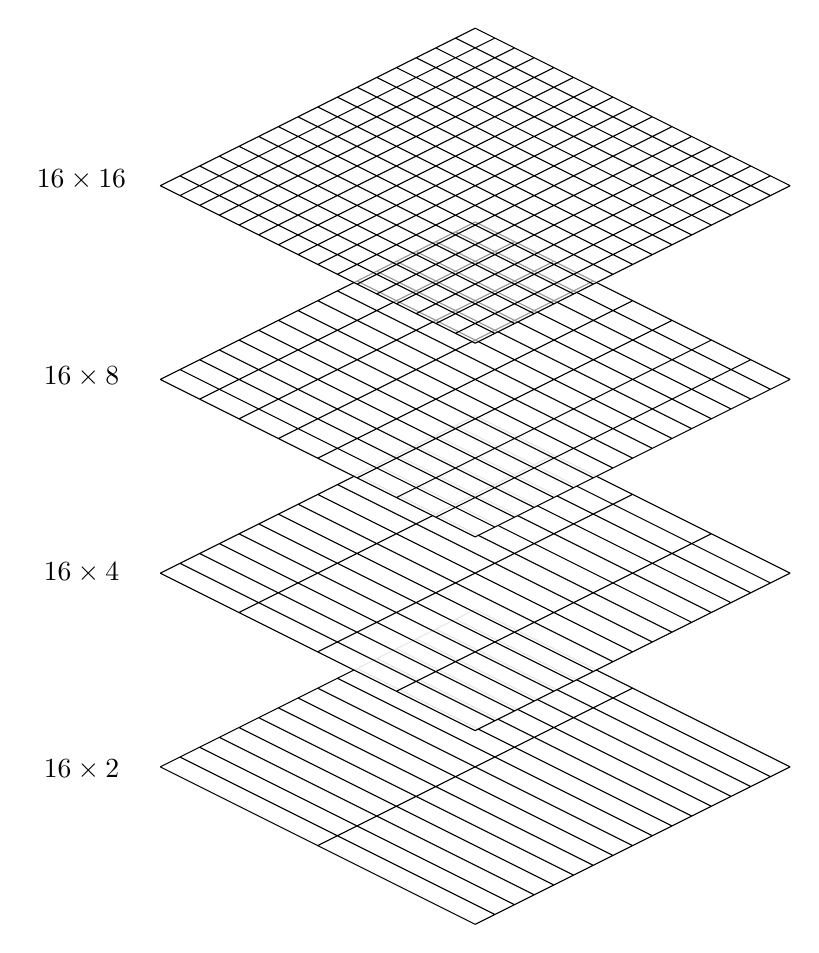
\begin{tikzpicture}

    % 16x2 Coarsest grid
    \node at (-5, -0.5) {$16\times2$};
    \begin{scope}[
            yshift=-70,every node/.append style={
            yslant=0.5,xslant=-1},yslant=0.5,xslant=-1
            ]
        \fill[white,fill opacity=0.9] (0,0) rectangle (4,4);
        \draw[xstep=2.5mm,ystep=20mm] (0,0) grid (4,4);
    \end{scope}

    % 16x4
    \node at (-5, 2) {$16\times4$};
    \begin{scope}[
        yshift=0,every node/.append style={
            yslant=0.5,xslant=-1},yslant=0.5,xslant=-1
                     ]
        \fill[white,fill opacity=.9] (0,0) rectangle (4,4);
        \draw[xstep=2.5mm,ystep=10mm] (0,0) grid (4,4);
    \end{scope}

    % 16x8
    \node at (-5, 4.5) {$16\times8$};
    \begin{scope}[
        yshift=70,every node/.append style={
        yslant=0.5,xslant=-1},yslant=0.5,xslant=-1
                     ]
        \fill[white,fill opacity=.9] (0,0) rectangle (4,4);
        \draw[xstep=2.5mm,ystep=5mm] (0,0) grid (4,4);
    \end{scope}

    % 16x16 Finest grid
    \node at (-5, 7) {$16\times16$};
    \begin{scope}[
        yshift=140,every node/.append style={
            yslant=0.5,xslant=-1},yslant=0.5,xslant=-1
          ]
        \fill[white,fill opacity=0.6] (0,0) rectangle (4,4);
        \draw[step=2.5mm] (0,0) grid (4,4);

    \end{scope}

\end{tikzpicture}

\end{document}
